\chapter{Проектирование ОЭП} 

\textit{Проектирование}~--- разработка проектной, конструкторской и другой технической документации, предназначенной для создания новых видов и образцов продукции промышленности.

\textit{Цель проектирования}~--- разработка нового изделия.

В процессе проектирования происходит поиск вариантов создания оптико-электронных приборов, его возможных конструкций, разработка и уточнение схем, теоретическое и экспериментальное исследование характеристик предполагаемых инженерных решений.

\textit{Конструирование} является составной частью проектирования и заключается в разработке конкретного варианта изделия на основе проведенных предварительных исследований. При этом создается конструкция проектируемого изделия: устройство, состав, взаимное расположение частей и элементов, способ их соединения и взаимодействия с учетом используемых материалов, технологии изготовления.

В процессе проектирования выпускают чертежи сборочных единиц и деталей, схемы, рассчитывают допуски на погрешности и технологию изготовления и сборки деталей, устанавливают технические условия на прибор, составляют техническое описание, разрабатывают другую конструкторскую документацию, необходимую для изготовления и эксплуатации изделия.

\section{Уровни проектирования}
Разработка сложных систем, какими являются ОЭП, проводится в определенной последовательности.

Отправной точкой создания любой системы являются выбор и формулировка цели проектирования. Необходимость создания нового изделия определяется как развитием конкретного направления техники, так и запросами потребителей (научных и производственных учреждений, человека-оператора). 

Обоснование исходных данных требует учета назначения системы, основных видов ее взаимодействия с другими системами или подсистемами, если она является подсистемой, входящей в состав другой более крупной системы, влияния внешних факторов.

В результате указанного рассмотрения должна быть получена полная совокупность исходных данных для проектирования прибора. 

Результатом проделанной работы является техническое задание~(ТЗ) на прибор, после утверждения которого можно переходить к собственно проектированию.

\newpage
Различают следующие основные уровни проектирования:
\begin{itemize}
	\item информационно-логический;
	\item системотехнический;
	\item схемотехнический;
	\item конструкторский;
	\item технологический.
\end{itemize}

Первые три уровня иногда объединяют в единый функциональный, или схемный уровень проектирования.
\begin{flushleft}
	\textbf{Информационно-логический уровень}
\end{flushleft}

В процессе проектирования на информационно-логическом уровне определяется конкретная структура данного прибора, определяются связи функциональных устройств между собой и устанавливаются требования технических заданий на проектирование отдельных функциональных устройств, исходя из требований ТЗ на прибор в целом. ТЗ на проектирование того или иного устройства содержит требования к сигналам, информации и командам, вырабатываемым этим устройством.

Таким образом, проектирование на этом уровне состоит из определения сначала структуры проектируемого объекта, а затем в определении оптимальных значений параметров этой структуры, т.е. составляющих ее элементов.

\begin{flushleft}
	\textbf{Системотехнический уровень}
\end{flushleft}

На системотехническом уровне функционального проектирования производится проектирование отдельных функциональных устройств, т.е. процесс разбивается на отдельные ветви. Каждое из функциональных устройств рассматривается здесь как структура, состоящая из взаимосвязанных функциональных блоков. Процесс проектирования заключается в определении оптимального состава и параметров блоков, например, оптической системы, приемника излучения, электронного тракта, системы отображения.

Все эти отдельные блоки рассматриваются на этом уровни как преобразователи сигналов, безотносительно к их внутреннему устройству. Здесь определяются требования к преобразованию сигналов тем или иным блоком, т.е. к его передаточным и прочим характеристикам.
\begin{flushleft}
	\textbf{Схемотехнический уровень}
\end{flushleft}

На схемотехническом уровне производится проектирование отдельных блоков, входящих в состав функциональных устройств, в соответствии с техническими заданиями, определенными на предыдущем уровне.

Каждому блоку соответствует своя ветвь, причем, начиная с этого уровня, различные ветви имеют различную «специализацию» в соответствии с физической природой блоков, игнорируемой на предыдущем уровне.

Схемотехнический уровень является важнейшим при функциональном проектировании.\\ В настоящее время он занимает наибольший объем работы и именно на этом уровне определяются основные параметры различных схем прибора, в конечном итоге обеспечивающие правильную работу прибора в соответствии с техническим заданием. Например, на этом уровне выделяется оптическая ветвь и производится расчет оптической системы прибора.

Целью проектирования оптической системы на этом уровне является определение как ее структуры, т.е. количества входящих в нее элементов и их типов, так и численных значений параметров этих элементов.

На электронной ветви схемотехнического уровня производится проектирование электронных схем блоков, преобразующих сигналы. Здесь, как и на оптической ветви, определяется структура схемы, т.е. состав и соединения ее функциональных элементов (резисторов, конденсаторов, транзисторов, интегральных схем), а затем и значения их параметров.

На механической ветви производятся аналогичные действия по проектированию кинематической схемы какого-либо устройства прибора.

Таким образом, в процессе схемотехнического проектирования разработчик определяет элементную базу будущего прибора.

Как показывает практика, очень часто проектирование новых элементов на этом уровне не требуется, и работа сводится к подбору элементов из имеющихся стандартных или покупных.

Рассмотренные уровни функционального проектирования являются типичными для ОЭП средней сложности. В более простых случаях некоторые уровни могут исключаться, например, информационно-логический или системотехнический.

\begin{flushleft}
	\textbf{Конструкторский уровень}
\end{flushleft}

Конструкторское проектирование, или просто конструирование, идет обычно параллельно функциональному проектированию или с некоторым отставанием и является важнейшей ветвью процесса проектирования, поскольку именно здесь оптико-электронный прибор приобретает не только схемную, но и материальную (правда пока только в документации) реализацию. Разработчик, работающий на этом уровне, называется обычно просто конструктором. 

В большинстве проектных организаций эти два уровня проектирования выполняются разными людьми и даже разными подразделениями. Так, например, проектирование оптической системы (оптической схемы) прибора выполняет обычно оптик-расчетчик или оптик-вычислитель, работающий в специализированном оптическом вычислительном бюро. Результатом этого проектирования является оптический выпуск, содержащий всю необходимую информацию об оптической схеме, включая ее параметры и их допустимые отклонения. 

На основании этой информации другой разработчик --- конструктор оптик-механик --- выполняет конструирование соответствующего оптического узла, например, объектива, диафрагм, механизма фокусировки объектива. Он выпускает чертежи всех деталей этого объектива, включая оптические сборочные чертежи отдельных узлов и объектива в целом.

Естественно, что этот процесс может быть итерационным. Так, в случае, если конструктору никак не удается надежно закрепить какую-либо оптическую деталь из-за неудачных с конструктивной точки зрения ее параметров, например, слишком крутых радиусов кривизны, приходится возвращаться на ветвь функционального проектирования и пересчитывать оптическую схему с изменением ее параметров.

Аналогичная картина наблюдается для электронных и кинематических схем. После того, как они разработаны на уровне функционального проектирования, конструктор материализует эти схемы в виде определенного монтажа на печатной плате, в виде деталей и узлов механизма.

Конструирование, также как и функциональное проектирование, разделяется на уровни.

Верхний уровень -- это компоновочный, на котором определяется общая компоновка всего прибора, взаимное расположение его отдельных узлов.

Один или несколько следующих уровней, в зависимости от сложности прибора --- это уровни узлов (сборочных единиц), где разрабатываются конструкции отдельных частей прибора. Сразу за компоновочным уровнем процесс конструирования может разделяться на ветви, соответствующие различным узлам, например: механическим, оптико-механическим, электронным или электромеханическим узлам. И, наконец, последний уровень --- это уровень деталей, на котором разрабатываются и выпускаются рабочие чертежи отдельных деталей.

\newpage
\begin{flushleft}
	\textbf{Технологический уровень}
\end{flushleft}

На уровне технологического проектирования производится разработка технологических процессов изготовления прибора. Как и на других стадиях разработки, здесь выделяются различные уровни:
\begin{itemize}
	\item верхний уровень -- испытание прибора (методики испытаний);
	\item уровень юстировки прибора (достижение верного взаиморасположения элементов);
	\item уровень сборки всего прибора;
	\item техпроцессы сборки, юстировки, контроля сборочных единиц;
	\item техпроцессы изготовления деталей. 
\end{itemize}

Верхним уровнем является уровень испытаний прибора, на котором разрабатываются методики испытаний прибора на соответствие различным пунктам ТЗ.

Следующим идет уровень юстировки, где разрабатываются методики юстировки прибора.

Затем уровень сборки всего прибора, который разветвляется по отдельным узлам (сборочным единицам). На этих уровнях разрабатываются техпроцессы сборки, юстировки и контроля различных сборочных единиц прибора. Наконец, на низших уровнях разрабатываются технологические процессы изготовления отдельных деталей.

Результатами работы на ветви технологического проектирования являются технологические карты, методики юстировки и контроля.

\section{Проектирование с использованием системного подхода}
Сущность системного подхода состоит в том, что объект проектирования рассматривается как система, т.е. как единство взаимосвязанных элементов, которые образуют единое целое и действуют в интересах реализации единой цели. 

Системный подход включает в себя выявление структуры системы, типизацию связей, определение свойств (атрибутов) системы, анализ влияния внешней среды, он требует рассматривать каждый элемент системы во взаимосвязи и взаимозависимости с другими элементами, вскрывать закономерности, присущие данной конкретной системе, выявлять оптимальный режим ее функционирования. 

Системный подход проявляется прежде всего в попытке создать целостную картину исследуемого или управляемого объекта. Исследование или описание отдельных элементов при этом производится с учетом роли и места элемента во всей системе.

Процесс функционирования сложной системы происходит на многих уровнях. Система расчленяется на подсистемы, которые представляют собой компоненты, необходимые для существования и действия системы.

Методическим средством реализации системного подхода к проектированию служит системный анализ, под которым понимается совокупность приемов и методов исследования объектов (процессов) посредством представления их в виде систем и их последующего анализа.

Системный анализ предполагает системный подход и к изучению связей между элементами, между подсистемами и системой.
\newpage
В основе системного подхода лежат следующие основные принципы и положения:
\begin{enumerate}
	\item Принцип цели: при разработке конструкции исходят из необходимости учета требований и показателей, которые должны быть реализованы. Должна быть ясна цель проектирования.
	\item Принцип целостности: объект рассматривается как единая система, состоящая из устройств, сборочных единиц элементов, функциональных устройств.
	\item Иерархичность строения: всякая система допускает разделение на подсистемы, что приводит к ступенчатости конструкции. Выявление и представление иерархии структуры объекта проводится с целью установления связей между частями объекта.
	\item Необходимо обобщение опыта и оценка перспектив развития систем данного или близких классов.
	\item Всестороннее рассмотрение взаимодействия системы с внешней средой и учет основных видов взаимодействия элементов и узлов внутри системы.
	\item Выбор критерия и показателей качества. Установление перспектив развития объектов.
	\item Правильное сочетание различных методов проектирования, в первую очередь, математических, эвристических и экспериментальных. Итерационный метод проектирования.
\end{enumerate}

\section{Блочно-иерархический подход к проектированию}
Если в системном подходе прибор рассматривается как сложная система, состоящая из связанных и взаимодействующих частей, то при блочно иерархическом подходе прибор рассматривается как иерархическая структура, состоящая из большого количества уровней и ветвей, наподобие некоторого опрокинутого дерева (рис.~\ref{pic:2block}).
\begin{figure}[H]
	\caption{Блочно-иерархическая структура}
	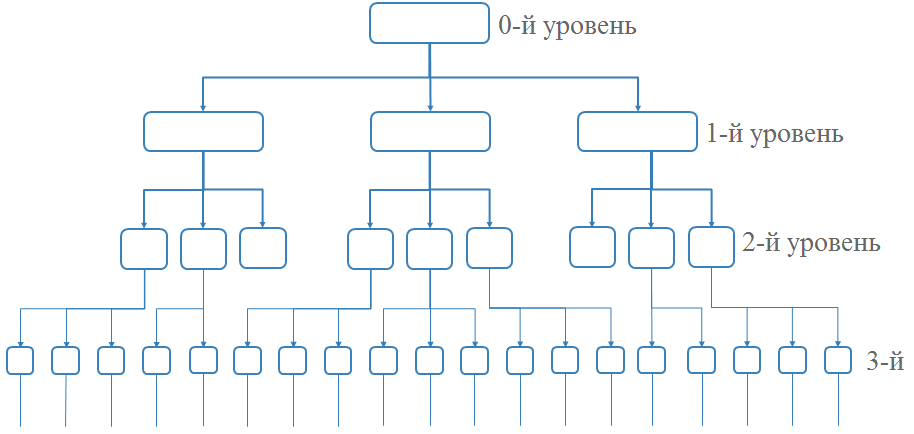
\includegraphics[width=1\textwidth]{2block.png}
	\label{pic:2block}
\end{figure}

В соответствии с блочно-иерархическим подходом в объекте проектирования может быть выделен ряд иерархических уровней (рис.~\ref{pic:2block}). На верхнем уровне подлежащий проектированию сложный объект состоит из ряда менее сложных элементов (например, для ОЭП -- приемная система, электронный блок обработки сигналов с выхода приемника излучения). Указанные элементы на более низком иерархическом уровне, в свою очередь, являются системами элементов менее сложной структуры (например, в приемную оптическую систему могут входить объектив, компенсатор, анализатор изображения, сканирующий блок). 

Далее подобное разделение на элементы может продолжаться до некоторого уровня, на котором дальнейшее разделение становится уже невозможным. Элементы, полученные на этом уровне, по отношению к объекту проектирования являются базовыми. Применительно к ОЭП такими базовыми элементами будут детали (оптические, механические) и различные комплектующие изделия (электро- и радиоэлементы, подшипники, электродвигатели).

Иерархия составных частей ОЭП при блочно-иерархическом подходе:
\begin{enumerate}
	\item Приборное устройство (или его конструируемая часть).
	\item Функциональная единица.
	\item Сборочная единица --- изделие, составные части которого подлежат соединению между собой сборочными операциями.
	\item Детали --- изделие, изготовленное из однородного (по наименованию и марке) материала без применения сборочных операций. (Или неделимые однородные тела, состоящие из элементов формы (геометрических поверхностей тел) и материала).
\end{enumerate}

Общий процесс проектирования при таком подходе представляется в виде движения по рассматриваемому дереву, при котором выполняются элементарные проектные операции на каждом уровне и на каждой ветви, т.е. структура проектирования также является блочно-иерархической, причем на каждом уровне и ветви процесс проектирования имеет дело с небольшим количеством элементов, рассматриваемых как целые, благодаря чему этот процесс достаточно несложен и вполне реализуем при нормальных ресурсах. Весь процесс проектирования, сплетающийся в виде блочно-иерархической структуры таких элементарных процессов, также теперь становится вполне реализуемым.

Такая структура позволяет осуществлять общий процесс проектирования, используя различные направления движения по блочно-иерархическому дереву. В зависимости от направления движения различают нисходящее, восходящее и смешанное проектирование.

Нисходящее проектирование, как следует из его названия, начинается с верхнего уровня, где прибор рассматривается как целое, затем проектируется его структура первого уровня, затем второго. Результатом проектирования на данном уровне является техническое задание для проектирования на следующем, более низком уровне.

Нисходящее проектирование всегда гарантирует выполнение требований технического задания на каждом уровне и поэтому должно бы считаться наиболее рациональным, но на каком-то уровне процесс проектирования может остановиться из-за того, что при существующих физических, технических, технологических или экономических ограничениях решение обратной задачи и соблюдение технического задания данного уровня становится невозможным. 

В этом случае приходится возвращаться на предыдущий уровень или даже выше, искать там другое решение своей обратной задачи, а затем опять пробовать вернуться на тот уровень, на котором процесс остановился, но с уже другим техническим заданием. Таким образом, блочно-иерархическая структура, позволяя в принципе реализовать процесс проектирования, делает неизбежным его итерационный характер, заключающийся в возврате к повторению проектирования на предыдущих уровнях с измененными условиями.

Восходящее проектирование выполняется в обратном порядке; при этом происходит как бы сборка отдельных узлов, а затем сборка всего прибора. Восходящее проектирование, как нетрудно увидеть, обычно гарантирует реализуемость проекта на любом уровне, но отнюдь не гарантирует соблюдения всех требований технического задания, поэтому процесс может остановится на каком-либо уровне из-за несоблюдения требований технического задания высшего уровня. При этом необходим возврат на предыдущие низшие уровни с попыткой <<собрать>> структуру данного уровня из других элементов. Таким образом и восходящее проектирование также неизбежно имеет итерационный характер.

При смешанном проектировании по части ветвей мы имеем нисходящий процесс, а по части~-- восходящий, которые в определенных точках встречаются. Итерационный характер такого проектирования также очевиден.

Из рассмотренных процессов предпочтительным является все-таки нисходящее проектирование. На практике, особенно для сложных приборов, процесс проектирования носит обычно смешанный характер с преобладанием нисходящих потоков, а восходящее проектирование применяется к тем частям приборов, которые собираются из стандартных, хорошо отработанных деталей, элементов и узлов.

Из рассмотренного становится ясен также эвристический характер проектирования, т.е. невозможность его полной алгоритмизации, автоматизации, поскольку ввиду сложности процесса и невозможности заранее определить полностью его ход необходимо принимать решения на основании опыта, интуиции, с привлечением творческих способностей разработчика, т.е. на базе так называемого алгоритма принятия решения. 

Все этапы проектирования выполняются на основе ТЗ. В случае, когда проектирование объекта проводится по сформулированным на более высоком иерархическом уровне ТЗ, оно носит название внутреннего. Внешнее проектирование предполагает разработку ТЗ на систему высшего иерархического уровня. При внешнем проектировании необходим правильный учет современного состояния техники, возможностей технологии, перспектив их развития, экономических факторов.